\documentclass{article}

\usepackage{amsmath, graphicx}
\graphicspath{ {./images/} }

\title{HW 10.4 Solutions}
\author{Principles of Microeconomics}
\date{\today}

\begin{document}

\maketitle

\subsection*{Mankiw}

\begin{enumerate}
\setcounter{enumi}{8}

\item 	

	\begin{enumerate}
	
	\item The value each firm places on a permit is equal to the cost the permit saves them by allowing them to pollute. That means Firm B values them the most and C the least. Firm B buys all of Firm C's permits for some price between \$10 and \$30 because Firm B is willing to pay more than the \$10 value that Firm C places on the permits. After buying 20 permits, Firm B can continue to produce its original 40 units of pollution, so it doesn't buy any more from Firm A. As a result, Firm A keeps its 20 permits. 

Since Firm C ends up with no permits, they spend $20 \cdot \$10 = \$200$ reducing their pollution. Since Firm A ends up with 20, they spend $10 \cdot \$20 = \$200$ reducing their pollution. Since Firm B ends up with 40 permits, they don't reduce their pollution. That means the total cost is \$400.

	\item Firm A would have spent $10 \cdot \$20 = \$200$ reducing their pollution. Firm B would have spent $20 \cdot \$30 = \$600$ reducing their pollution. Firm C would have spent \$0 reducing their pollution because they would have enough permits to cover their pollution. That means the total cost would be \$800.

	\end{enumerate}

\end{enumerate}

\subsection*{Non-Mankiw}

\begin{enumerate}
	
\item

	\begin{enumerate}
	
	\item
		\begin{align*}
		50P_{mkt} &= 200 - 50P_{mkt} \\
		100P_{mkt} &= 200 \\
		P_{mkt} &= 2 \\
		Q_{mkt} &= 50(2) \\
		&= 100
		\end{align*}
		
	\item
		\begin{align*}
		50(P_{optimum}-2) &= 200 - 50P_{optimum} \\
		100P_{optimum} &= 300 \\
		P_{optimum} &= 3 \\
		Q_{optimum} &= 200 - 50(3) \\
		&= 50
		\end{align*}
		
		\begin{center}
		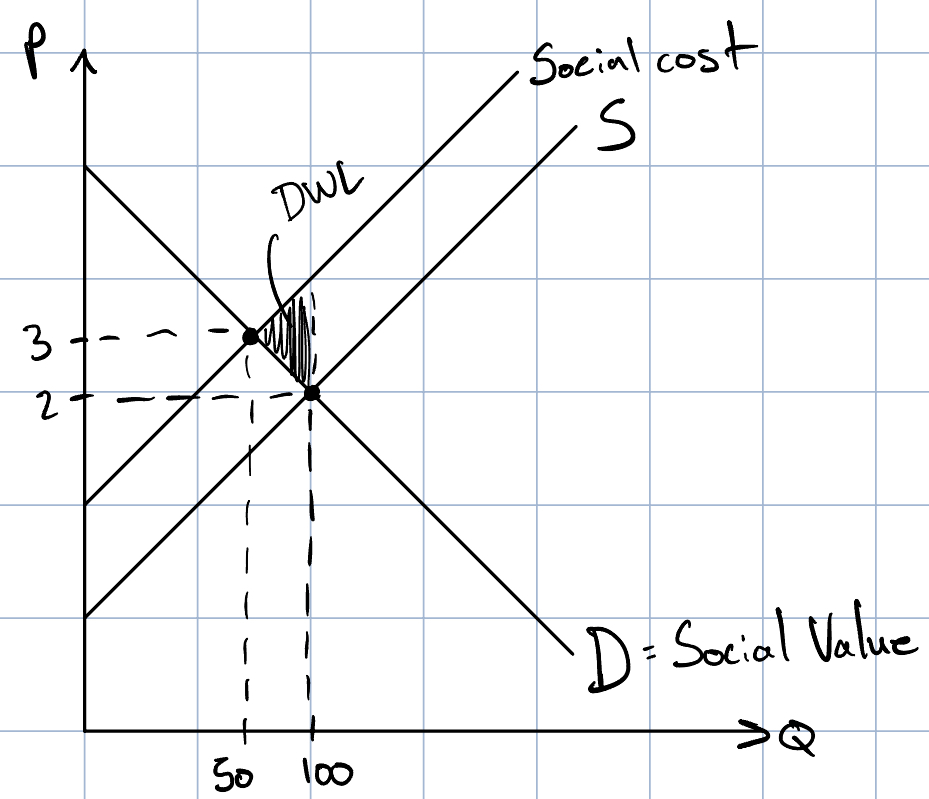
\includegraphics[width = 0.5\textwidth]{q1b}
		\end{center}
		
	\item Yes, there is dead weight loss because too many toys are made. Buyers and sellers have no incentive to consider the external costs the toys create for others, so they supply and demand too many of them. 
	
	\end{enumerate}

\item

	\begin{enumerate}
	
	\item The neighbors will pay Tyson between \$50,000 and \$100,000 to deal with the waste in a cleaner way. That's because the neighbors value clean air and water more than it costs Tyson to deal with its waste cleanly. That means the neighbors and Tyson can agree on a deal that's mutually beneficial where the neighbors spend less than their willingness to pay for clean air and water, and Tyson receives more than their cost of dealing with their waste cleanly. 
	
	\item Tyson will deal with its waste cleanly. Tyson won't offer the neighbors more than \$50,000 to avoid dealing with its waste cleanly. The neighbors won't accept an offer for less than \$100,000. As a result, they won't come to a deal.
	
	\item The neighbors will pay Tyson between \$60,000 and \$90,000 to deal with the waste in a cleaner way. Because of the \$10,000 attorney fee, it now costs Tyson a total of \$60,000 to negotiate with the neighbors and then deal with the waste cleanly. The neighbors are willing to pay them up to \$90,000 because they also have to pay the \$10,000 attorney fee, and they're only willing to pay \$100,000 total for clean air and water. At any price between \$60,000 and \$90,000, they can come to a mutually beneficial deal. 
	
	\end{enumerate}

\end{enumerate}

\end{document}